
\section{Sonars}
The sonar sensors where already present on WTR, but the implementation lacked professionalism and long term stability was at risk, at mechanical, electrical, and software level.
The improvements are described in each of these aspects in the following sections.

\subsection{Mechanical setup}
Instead of tie wraps and tape, a special clamp, ball joint, and housing for the HC-SR04 was designed in solidworks and 3D printed. See figure below.
There are eight sensors which are strategically placed around WTR.
The clamp (orange) is designed to fit around the 25mm square tubes which are present around WTR. 
This clamp is provided with an opening which will hold the ball clamp (red).
The ball (green) can be pressed into the ball clamp easily and will create a ball joint mechanism.
The ball is provided with a tapered shaft which is pressed into the housing (blue).
The housing holds the sonar sensor, and is closed with a lid (grey).

\begin{figure}[H]
\centering
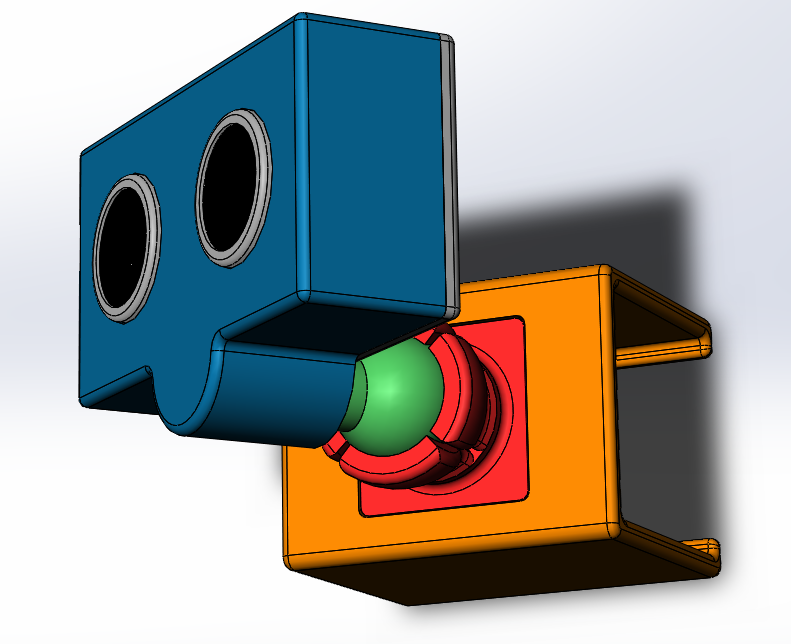
\includegraphics[width=12cm]{SonarSensorAssembly.png}
\caption{Sonar sensor assembly}
\label{fig::sonarassembly}
\end{figure}


\subsection{Electrical setup}
Instead of breadboards and a lot of loose wires a special cable was designed. 
This cable is split into two sections, one for the three front sensors and the other for the five sensors on the back of WTR.
The sections meet in the middle and connect to an arduino Uno.
The sections contain the common power wires, the common trigger wire and individual echo wires.
The cable is made from flat cable and provided with connectors which makes repairing or replacing separate parts easier.

The wiring for the sonar sensors can be found in the schematic \ref{fig::wiringsonar}.

\begin{figure}[H]
\centering
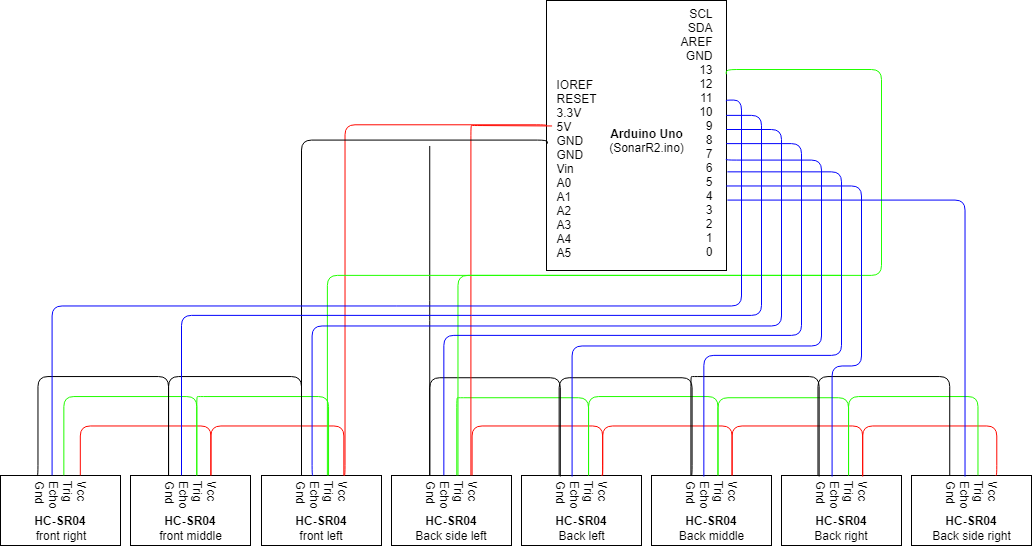
\includegraphics[width=12cm]{SonarDiagram.png}
\caption{Wiring setup for the 8 sonar sensors to Arduino communication}
\label{fig::wiringsonar}
\end{figure}

 
\newpage    